\documentclass[10pt]{standalone}
\usepackage{amsmath}
\usepackage{amssymb}
\usepackage{pgf,tikz,pgfplots}
\usepackage{mathrsfs}
\usetikzlibrary{arrows}
\pagestyle{empty}
\usepackage{siunitx}

\pgfkeys{/pgfplots/Axis Style/.style={
		grid,
		% width=13.5cm, height=5cm,
		xlabel={$t$},
		ylabel={$y$},
		xlabel style={below left},
		ylabel style={below left},
		axis x line=center, 
		axis y line=middle, 
		samples=100,
		ymin=-3, ymax=3,
		xmin=0, xmax=3.5,
		domain=0:pi
	}}

\begin{document}
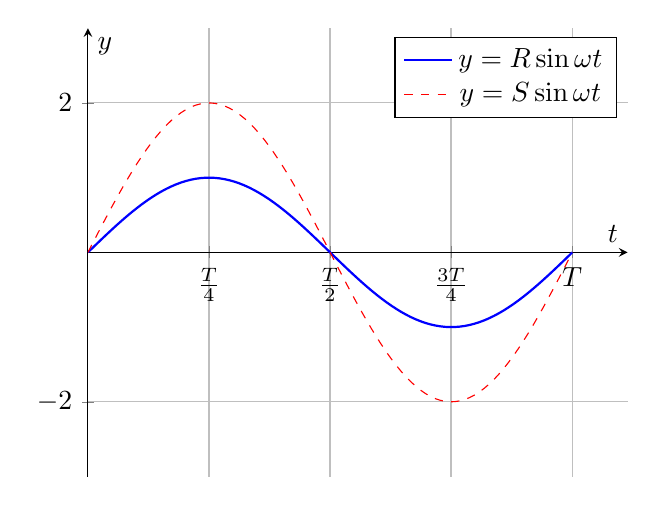
\begin{tikzpicture}%[>=triangle 45]
\begin{axis}
[
    Axis Style,
    xtick={
    	0, 0.785, 1.57, 3.14,2.355,6.28
    },
    xticklabels={
    	$0$, $\frac{T}{4}$,  $\frac{T}{2}$,
    	$T$, $\frac{3T}{4}$, $T$
    },
    legend entries={{$y=R\sin\omega t$},{$y=S\sin\omega t$}},
    % ytick=\empty, % That's the trick 
  %  yticklabels={,,},
%     ytick={
%     	-2,-1,0,1,2
%     },
%     yticklabels={
%     $-R$,$-1$,$0$,$+1$,$R$
%     }
]
\addplot [mark=none, thick, blue] {sin(deg(2*x))};
\addplot [mark=none,  dashed, red] {2*sin(deg(2*x))};
\end{axis}
\end{tikzpicture}

\end{document}